% TeX encoding = utf8
% TeX spellcheck = pl_PL 
\documentclass[a4paper, 12pt]{article}
\usepackage[utf8]{inputenc}
\usepackage[polish]{babel}
\usepackage{polski}
\usepackage{float}
\usepackage{graphicx}
\usepackage{listings}
\usepackage{amsfonts}
\usepackage{geometry}
\usepackage{indentfirst}
\usepackage{subfigure}
\usepackage{url}
\usepackage{listings}
\usepackage{color}
\usepackage[usenames,dvipsnames]{xcolor}
\usepackage{amsmath}

%\renewcommand*{\addcontentsline}[3]{\addtocontents{#1}{\protect\contentsline{#2}{#3}{}}}
\newgeometry{tmargin=2.5cm, bmargin=2.5cm, lmargin=3.5cm, rmargin=2.5cm}
%\setcounter{secnumdepth}{2}
\setlength{\fboxsep}{0pt}
\lstset{
	basicstyle=\footnotesize\ttfamily,
	breaklines=true,
	language=Python,
	breakatwhitespace=true,
	frame=leftline,
	numbers=left,
	numberstyle=\tiny,
	commentstyle=\color{Gray}\footnotesize\ttfamily}


\author{Anna Wujek \\ Łukasz Korpal \\ Wiktor Ślęczka}
\title{Roboty monitorujace skażenie środowiska - symulator V-REP}
\date{10 czerwca 2016}


\begin{document}
	\sloppy
	\maketitle
	\newpage
	\tableofcontents
	\newpage
	\section{Zadanie}
	Celem projektu było stworzenie symulatora mobilnej sieci ad hoc (MANET) do monitorowania skażenia środowiska naturalnego. Węzłami sieci są roboty mobilne, wyposażone w czujniki oraz komunikujące się między sobą. Zadaniem robotów jest lokalizacja chmury skażenia i otoczenie jej robotami, monitorującymi jej położenie i granice, przy założeniu utrzymania spójności sieci.
	
	
	\section{Projekt systemu}
	\subsection{Założenia}
	\begin{itemize}
		\item Roboty potrafią się na bieżąco lokalizować.
		\item System składa się z pewnej liczby robotów mobilnych.
		\item Roboty mobilne działają autonomicznie i potrafią same zorganizować sieć.
		\item Roboty są wyposażone w czujniki pozwalające im wykrywać poziom skażenia oraz przeszkody.
		\item Roboty są wyposażone w urządzenia pozwalające im się między sobą komunikować się między sobą.
		\item Chmura skażenia jest odgórnie określona i niezmienna w trakcie trwania symulacji.
		\item Nieznana jest mapa obszaru poszukiwań, ale znane są jego granice i kształt - prostokąt.
	\end{itemize}
	
	\subsection{Scenariusz działania}	
		
		Algorytm realizowany przez każdego robota:
		\begin{enumerate}
		\item Warunek początkowy: robot znajduje się w dowolnym punkcie przestrzeni na mapie. Z punktu tego musi istnieć droga prowadząca do obszaru poszukiwań.
		\item Przemieść się do punktu początkowego (rys. \ref{plansza}), zależnego od liczby robotów, wymiarów przestrzeni poszukiwań i zasięgu czujników (rys. \ref{odleglosci}), zgodnie ze wzorem:		
		\begin{eqnarray}
		x &=& -length / 2 \\
		y &=& width / 2 + distance * robot\_number + distance / 2 \nonumber
		\end{eqnarray}
		W obliczeniach wykorzystywane są następujące parametry:
		\begin{eqnarray}
		max\_spaces &=& sensor\_range \cdot precision\_range\nonumber \\
		no\_stages &=& ceil(width / (max\_spaces \cdot no\_robots))\nonumber\\
		spaces\_width &=& width / no\_stages\nonumber\\
		distance &=& spaces\_width/no\_robots\nonumber
		\end{eqnarray}
		\begin{figure}[h!]
			\centering
			\includegraphics*[width=0.7\columnwidth]{img/plansza.pdf}
			\caption{Ustawienie początkowe robotów}
			\label{plansza}
		\end{figure}
		\begin{figure}[h!]
			\centering
			\includegraphics*[width=0.7\columnwidth]{img/odleglosci.pdf}
			\caption{Sposób ustawienia robotów w szeregu}
			\label{odleglosci}
		\end{figure}
		\item Wyznacz kolejny punkt docelowy, zgodnie ze wzorem:
		\begin{eqnarray}
		x_n &=& direction \cdot length / 2 + direction + substage\_length \cdot substage\nonumber\\
		y_n &=& width / 2 + distance \cdot robot\_number + stage \cdot spaces\_width + distance / 2\nonumber
		\end{eqnarray}
		\item Udaj się do punktu docelowego, monitorując skażenie oraz wykrywając przeszkody.
		\item Jeśli wykryto przeszkodę, omiń ją algorytmem Bug2. Wyznacz następny punkt docelowy, jest aktualny został minięty.
		\item Jeśli wykryto chmurę skażenia, zatrzymaj się.
		\item Jeśli cały obszar poszukiwań sprawdzony, to koniec algorytmu; jeśli nie, to przejdź do punktu 3.
		\end{enumerate}
		\begin{figure}[h!]
			\centering
			\includegraphics*[width=0.7\columnwidth]{img/ruch.pdf}
			\caption{Ruch szeregu robotów}
			\label{ruch}
		\end{figure}
		
	
	\subsection{Struktura systemu}
	System prezentowany w projekcie składa się z następujących elementów:
	\begin{itemize}
	\item symulator przestrzeni roboczej	
	\item symulator robotów
	\item symulator chmury skażenia	
	\item komunikacja
	\end{itemize}
	
	\subsubsection{Symulator przestrzeni roboczej}
	Symulator ten jest odpowiedzialny za wizualizację całej symulacji - przestrzeni roboczej, przeszkód, robotów oraz chmury skażenia. Generuje także fizyczne oddziaływania między elementami, np. kolizje oraz odczyty czujników (oprócz czujników skażenia). Pożądane jest wykorzystanie w tym celu gotowego narzędzia, oferującego modele robotów i czujników, silnik fizyczny oraz interfejsy komunikacyjne.
	
	Narzędziem wykorzystanym w projekcie był symulator V-Rep. Jest on dedykowany do tego typu symulacji i spełnił postawione założenia. W projekcie symuluje rzeczywiste receptory (czujniki odległości) i rzeczywiste efektory (silniki robotów) systemu, a także pełni rolę wirtualnego efektora (warstwy pośredniczącej między rzeczywistym efektorem a podsystemem sterowania, przekładającej polecenia sterowania na uruchamianie silników, a tym samym ruch robota).
	
	\subsubsection{Symulator chmury skażenia}
	Symulator ten jest odpowiedzialny za generowanie odczytów czujników skażenia. Odczyt jest obliczany na podstawie założonego wcześniej kształtu chmury oraz sposobu, w jaki skażenie rośnie wgłąb chmury. Ze względu na brak możliwości zaimplementowania tego typu obiektu bezpośrednio w wybranym symulatorze V-Rep, chmura skażenia została zasymulowana osobno. W projekcie pełni rolę wirtualnego receptora (warstwy pośredniczącej między rzeczywistym receptorem -- czujnikiem skażenia -- a podsystemem sterowania), interpretującego odczyt czujnika skażenia.
	
	\subsubsection{Symulator robota}
	W systemie symulator ten będzie zwielokrotniony, aby uzyskać grupę kilku robotów. Odpowiedzialny jest za wyznaczanie sterowania robotów w zależności od odczytów z czujników i wewnętrznego imperatywu, czyli zadania, jakie roboty realizują.
	
	W projekcie pełni dwie bardzo ważne role: wirtualnego receptora (warstwy pośredniczącej między rzeczywistymi receptorami -- czujnikami odległości -- a podsystemem sterowania) interpretującego dane z czujników odległości (przetwarzanie polega na filtracji wyników i stwierdzeniu które pomiary są przydatne) oraz podsystemu sterowania (logiki robota, która na podstawie danych z wirtualnych receptorów podejmuje decyzje co do stanu i dalszego zachowania robota, a następnie wysyła odpowiednie sterowania do wirtualnego efektora; kolejnym zadaniem podsystemu sterowania jest komunikacja z innymi robotami w systemie).
	
	Każdy robot realizuje dokładnie ten sam algorytm - nie ma jednego wyróżnionego lidera.
	
	\subsubsection{Komunikacja}
	Aby cały system działał poprawnie, poszczególne elementy muszą móc się ze sobą komunikować. W systemie rozróżniamy następujące kanały komunikacyjne i przesyłane informacje:
	\begin{itemize}
	\item Symulator przestrzeni roboczej $\rightarrow$ Symulator robota:
		\begin{itemize}
		\item odczyty z czujników (oprócz czujnika skażenia)
		\item pozycja robota (położenie + orientacja)	
		\end{itemize}
	\item Symulator robota $\rightarrow$ Symulator przestrzeni roboczej:
		\begin{itemize}
		\item sterowanie poszczególnymi silnikami
		\end{itemize}
	\item Symulator chmury skażenia $\rightarrow$ Symulator robota:
		\begin{itemize}
		\item odczyt czujnika skażenia
		\end{itemize}
	\item Symulator robota $\rightarrow$ Symulator robota:
		\begin{itemize}
		\item ostatni punkt docelowy, do którego udało się dotrzeć
		\item informacja o wykrytej chmurze skażenia
		\end{itemize}
	
	\end{itemize}
	
	\begin{figure}[h!]
	\centering
	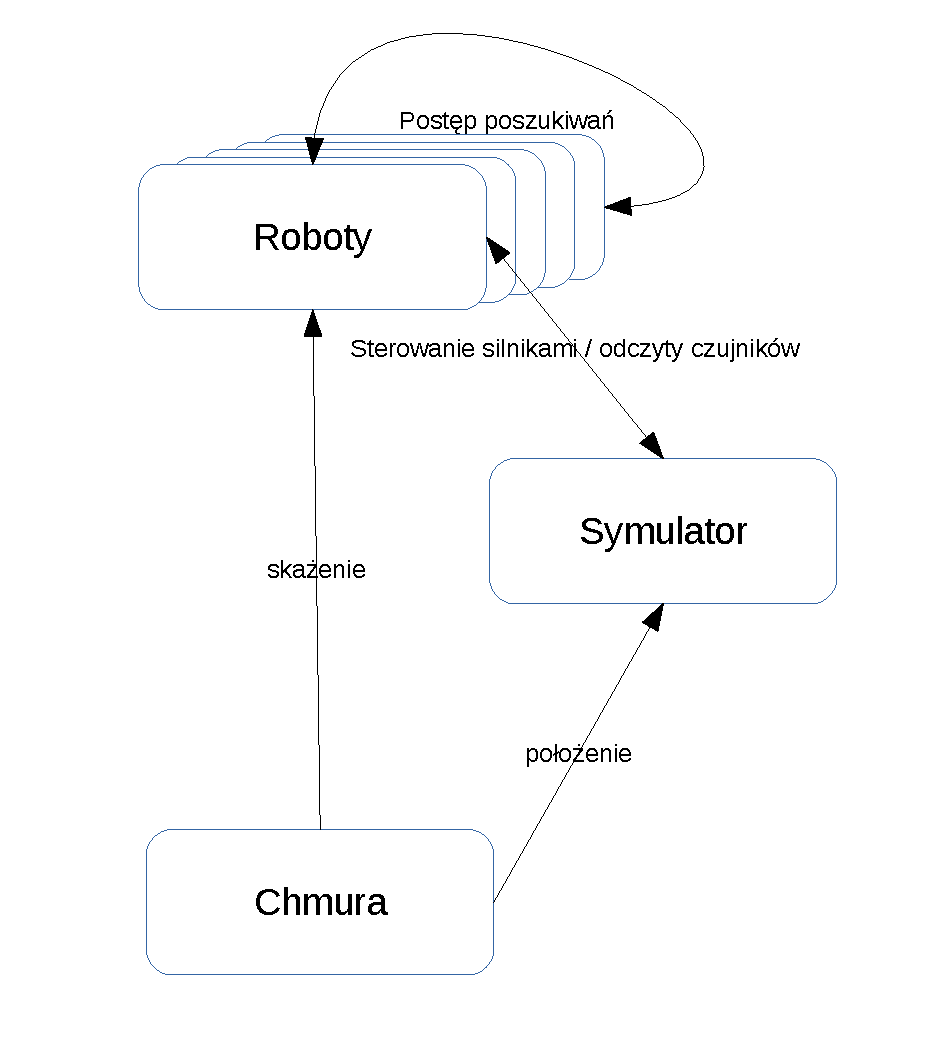
\includegraphics[width=0.6\columnwidth]{img/system.pdf}
	\end{figure}
	
	
	\subsection{Algorytmy}
		
		\subsubsection{Algorytm poszukiwania chmury}
		Roboty rozpoczynają pracę od ustawienia się w formacji linii. Następnie dla każdego robota wyznaczany jest następny punkt docelowy, do którego musi dojechać. Punkty docelowe wyznaczane są w taki sposób, aby roboty ponownie ustawiły się w linii. Po dojechaniu do punktu docelowego robot wysyła informację o tym zdarzeniu do innych robotów. Linia punktów docelowych jest jednocześnie miejscem synchronizacji - jeśli jakiś robot jechał wolniej (np. z powodu omijania przeszkody), to reszta na niego czeka. Powoduje to wolniejsze przeszukiwanie, ale zapewnia spójność sieci -- robot nigdy nie jest oddalony od swoich sąsiadów bardziej, niż odległość do następnego punktu docelowego. Odległość ta dobrana jest w taki sposób, aby spójność sieci została zachowana.
		
		Roboty w ten sposób poruszają się do przodu do momentu dotarcia do przeszkody, toksycznej chmury lub granicy obszaru poszukiwań. W przypadku powyższych wydarzeń, uruchamiane są odpowiednie algorytmy.
		
		Gdy roboty dotrą do końca obszaru poszukiwań, zatrzymują się, przesuwają w bok i kontynuują poszukiwania w drugą stronę, granicząc z poprzednim obszarem poszukiwań -- w ten sposób szerokimi pasami przeszukują cały obszar mapy.
		
		\subsubsection{Algorytm bug 2}
		Algorytm ten jest stosowany w przypadku napotkania przeszkody przez robota. Polega on na podążaniu wzdłuż ściany przeszkody do momentu osiągnięcia punktu leżącego za napotkaną ścianą, na przedłużeniu początkowej ścieżki ruchu. Jego działanie zostało przedstawione na rysunku \ref{bug2_img}.
		\begin{figure}[h!]
			\centering
			\includegraphics*[width=0.7\columnwidth]{img/40-0.png}
			\caption{Działanie algorytmu bug 2}
			\label{bug2_img}
		\end{figure}

		\subsubsection{Algorytm otaczania chmury}
		W momencie napotkania chmury przez któregokolwiek robota, zatrzymuje się on (po osiągnięciu natężenia toksyn określonego arbitralnie). Pozostałe roboty jadą dalej, po łuku -- tak, aby nie przerwać połączenia z siecią. Gdy napotkają określone stężenie chmury, zatrzymują się. Gdy wszystkie roboty zatrzymały się, zwracają się w jedną stronę i zaczynają okrążać chmurę, utrzymując się na granicy stężenia oraz zachowując spójność sieci. Jego działanie przedstawiono na rysunku \ref{otaczanie}.
		\begin{figure}[h!]
			\includegraphics*[width=0.5\columnwidth]{img/chmura/1.png}
			\includegraphics*[width=0.5\columnwidth]{img/chmura/2.png}
			\includegraphics*[width=0.5\columnwidth]{img/chmura/3.png}
			\includegraphics*[width=0.5\columnwidth]{img/chmura/4.png}
			\caption{Działanie algorytmu otaczania chmury. Robot 2 napotyka chmurę, pozostałe roboty zbliżają się do chmury aż do wartości granicznej, następnie cała sieć zaczyna krążyć wokół chmury, monitorując jej kształt i położenie.}
			\label{otaczanie}
		\end{figure}
		
		
		
	
	
	
	\section{Realizacja}
	\subsection{Plik konfiguracyjny}
	Plik konfiguracyjny powinien zawierać informacje o planszy, robotach i chmurze -- w trzech rozdzielonych modułach.
	\begin{itemize}
	\item Moduł [board] opisuje wielkość sektora poszukiwań.\\
		Posiada następujące parametry:
	\begin{itemize}
	\item width -- szerokość planszy
	\item length -- długość planszy
	\end{itemize}
	\item Moduł [robots] opisuje roboty biorące udział w symulacji.\\
		Posiada następujące parametry:
	\begin{itemize}
	\item count -- liczba robotów
	\item sensor\_range -- zasięg czujników toksyczności
	\item precision\_range -- parametr wymaganej precyzji, ogranicza maksymalny zasięg czujników, wpływając na mniejsze odległości między robotami (zwiększa zmienną P, por. rys. \ref{odleglosci})
	\end{itemize}
	\item Moduł [cloud] opisuje położenie i wielkość chmury.\\
		Posiada następujące parametry::
	\begin{itemize}
	\item center -- położenie środka chmury
	\item radius -- średnica chmury
	\end{itemize}
	\end{itemize}
	
	\subsection{Komunikacja}
	Komunikacja przebiega na zasadzie ogłaszania aktualnych informacji na swój temat przez roboty (oraz chmurę). Informacje przesyłane są za pomocą struktury JSON do gniazd, przypisywanych każdemu modułowi osobno.
	Wiadomości opatrzone są typem, pozwalającym sklasyfikować komunikat. Dane tworzone są w postaci usystematyzowanych słowników, których struktura została odgórnie ustalona.
	Komunikaty są wysyłane i odbierane asynchronicznie.
	\subsubsection{Roboty}
	Roboty wysyłają informacje o swoim postępie w wiadomościach typu "progress". Zawierają one następujące elementy:
	\begin{itemize}
	\item "robot" - numer identyfikacyjny robota
	\item "substage" - postęp robota wzdłuż wyznaczonej ścieżki
	\item "stage" - postęp robota w numerze ścieżki
	\end{itemize}
	Poniżej przedstawiono przykład tworzenia wiadomości o postępie robota.
	\begin{verbatim}
	    def broadcast_info(self):
	        message = str(self.robot._name)+str(self.substage)
	        message = dict()
	        message["robot"] = self.robot.name
	        message["stage"] = self.stage
	        message["substage"] = self.substage
	        message["type"] = "progress"
	        self.robot.commutron.broadcast(json.dumps(message))
	\end{verbatim}
	Dodatkowo, symulując działanie czujników toksyczności, wysyłają zapytania do procesu chmury o stężenie w swoim położeniu. Są to
	\subsubsection{Chmura}
	Skrypt odpowiadający za symulację chmury wysyła informację o jej położeniu do robotów w wiadomościach typu "cloudread".
	Zawierają one następujące elementy:
	\begin{itemize}
	\item "concentration" - stężenie toksycznych substancji
	\item "robot" - numer robota, z którym przebiega komunikacja
	\item "position" - pozycja robota
	\end{itemize}
	Poniżej przedstawiono przykład tworzenia wiadomości o chmurze.
	\begin{verbatim}
	        res = dict()
	        res['concentration'] = self.concentration(data["position"])
	        res['robot'] = data['robot']
	        res['position'] = data['position']
	        res['type'] = "cloudread"
	\end{verbatim}
	
	
	\subsection{Roboty}
	Wykorzystywane w realizacji zadania roboty Pionieer p3dx wyposażone w ultradźwiękowe czujniki odległości - będą one zapewnione przez symulator V-Rep. Posiadają one napęd różnicowy, pozwalający na dużą swobodę poruszania się po symulowanej przestrzeni.
	
	Roboty te mają napęd różnicowy, co pozwala im na obracanie się w miejscu. Dlatego też realizacja ruchu robota odbywa się poprzez zadanie punktu docelowego, a następnie takie sterowanie, aby dotrzeć do niego z dowolną orientacją. Do sterowania wykorzystane zostały dwa regulatory proporcjonalne, jeden odpowiedzialny za jazdę do przodu -- wolniej lub szybciej, w zależności od odległości od miejsca docelowego, drugi odpowiedzialny za obrót robota -- tak, aby robot był ustawiony przodem do miejsca docelowego. Złożenie tych dwóch ruchów pozwala na płynne i gładkie dojechanie do miejsca docelowego.
	
	Regulator odpowiedzialny za jazdę do przodu:
	
	\begin{eqnarray}
	u_{11}(k) &=& u_{12}(k) = K_1 \cdot e(k) \quad \text{jednakowe prędkości na oba koła}\nonumber \\
	e(k) &=& y_{zad}(k) - y(k) \nonumber \\
	K_1 &=& v_{max} \nonumber \\
	0 &\leq& u_{11}(k),u_{12}(k) \leq v_{max} \nonumber
	\end{eqnarray}
	gdzie:\\
	$u_{11}(k),u_{12}(k)$ -- sterowanie, czyli prędkości zadawane na oba koła\\
	$y_zad()$ -- współrzędne punktu docelowego\\
	$y(k)$ -- aktualne położenie robota\\
	$v_{max}$ -- maksymalna prędkość.
	
	Regulator odpowiedzialny za obrót robota:
	\begin{eqnarray}
	u_{21}(k) &=& -u_{22}(k) = K_2 \cdot e(k) \quad \text{przeciwne prędkości na oba koła}\nonumber \\
	e(k) &=& \theta(k)\nonumber \\
	K_2 &=& v_{max2} \nonumber \\
	0 &\leq& u_{21}(k),u_{22}(k) \leq v_{max2} \nonumber
	\end{eqnarray}
	gdzie:\\
	$u_{21}(k),u_{22}(k)$ -- sterowanie, czyli prędkości zadawane na oba koła\\
	$\theta()$ -- kąt pomiędzy kierunkiem jazdy robota, a prostą poprowadzoną przez robota i punkt docelowy (0, jeśli robot skierowany przodem do punktu docelowego)\\
	$v_{max2}$ -- maksymalna prędkość podczas obrotu.
	
	Sterowanie wysyłane do robota jest złożeniem tych dwóch ruchów:
	\begin{displaymath}
	V(k)=\begin{bmatrix}
	v_1(k), & v_2(k)
	\end{bmatrix}=\begin{bmatrix}
	u_{11}(k)+u_{21}(k), & u_{21}(k)+u_{22}(k)
	\end{bmatrix}
	\end{displaymath}
		
	
	Dodatkowo, czujniki stężenia toksycznych substancji będą realizowane w skryptach Pythona, ułatwiając jej symulację. Informacje o jej położeniu i kształcie będą przekazywane do V-Repa, gdzie nastąpi ich wizualizacja.
	
	
	\section{Wnioski}
	\subsection{Wykorzystane narzędzia}
	Symulator V-Rep okazał się narzędziem o wielu możliwościach, bardzo rozbudowanym i przydatnym, lecz także posiadającym ograniczenia:
	\begin{itemize}
		\item symulator posiada wiele gotowych modeli robotów przeznaczonych do różnego typu zadań i wyposażonych w czujniki; z drugiej strony tworzenie własnego modelu robota jest skomplikowane i czasochłonne, dlatego zdecydowaliśmy się na skorzystanie z gotowego modelu spełniającego nasze wymagania;
		\item program ten dobrze symuluje fizyczne oddziaływania (np. kolizje) oraz dane z czujników, jednak czasem zdarza mu się błędnie określić pozycję, orientację lub odczyt z czujnika odległości -- zdarzenia te są losowe i dość rzadkie, ale wpływają negatywnie na działanie algorytmów;
		\item zdecydowaną zaletą jest możliwość uruchomienia serwera, który pozwala na komunikację z symulatorem z zewnątrz, co wykorzystaliśmy w projekcie;
		\item program podczas symulacji wymaga dość dużej mocy obliczeniowej.
	\end{itemize}
	Podsumowując, jest to dobre narzędzie do niewielkich projektów i symulacji oraz nauki przed programowaniem prawdziwych robotów, lecz w przypadku dużych i skomplikowanych projektów może okazać się zbyt powolny i niestabilny.
	
	Oprogramowanie poza V-Repem było tworzone przy wykorzystaniu języka Python. Rozwiązanie to miało wiele zalet:
	\begin{itemize}
		\item tworzenie części systemu poza V-Repem umożliwiło skorzystanie z wielu bibliotek Pythona;
		\item każdy robot działał w osobnym wątku (podobnie chmura skażenia), dzięki czemu symulacja była bardziej zbliżona do rzeczywistości;
		\item wadą rozwiązania była konieczność komunikacji z V-Repem, która wprowadzała opóźnienia, częstotliwość odświeżania stanu robotów oraz symulacji w V-Repie się różniła, a komunikacja nie zawsze działała zgodnie z oczekiwaniami (np. w pewnym momencie pytając V-Repa o pozycję robota otrzymywaliśmy w odpowiedzi pozycję kamery).
	\end{itemize}
	
	\subsection{Realizacja założeń}
	
	\subsubsection{Symulacja środowiska i robotów}
	Udało się stworzyć symulację zawierającą grupę robotów mobilnych. Każdy robot składał się z:
	\begin{itemize}
		\item symulatora rzeczywistych efektorów i receptorów (realizowanych w V-Repie oraz w symulatorze chmury skażenia w Pythonie);
		\item wirtualnych efektorów i receptorów (realizowanych w V-Repie oraz w symulatorze robota w Pythonie);
		\item podsystemu sterowania (realizowanego w symulatorze robota w Pythonie).
	\end{itemize}
	Każdy model w V-Repie miał swój unikalny odpowiednik po stronie Pythona, z którym komunikował się na tyle często, by stan logiki robota i wizualizacja w V-Repie nie różniły się między sobą.	
	
	\subsubsection{Komunikacja}	
	
	Dzięki zaimplementowanej komunikacji między wątkami Pythona a V-Repem możliwe było określenie aktualnej pozycji i orientacji robota.
	
	Dzięki czujnikom odległości dostępnym w gotowym modelu oraz zamodelowanemu czujnikowi chmury skażenia możliwa była symulacja odczytów, na podstawie których robot podejmował decyzje. Symulacja wiernie odpowiadała rzeczywistości -- robot nie korzystał z żadnych danych, których by nie miał w rzeczywistości.
	
	Komunikacja między robotami, zrealizowana w całości po stronie Pythona, zapewniła zachowanie spójności sieci - roboty zawsze miały informację, na jakim etapie poszukiwań znajdują się inne jednostki.
	
	\subsubsection{Realizacja zadania poszukiwania chmury}
	Zaproponowany algorytm przeczesywania zadanego obszaru sprawdził się bardzo dobrze. Przeczesywanie obszaru poszukiwań szerokim pasem robotów jadących w linii daje gwarancję wykrycia chmury (nawet niewielkiej), a jednocześnie nie pozwala na utracenie spójności sieci, ponieważ całą linia robotów czeka na te, które jadą wolniej (podstawą do zachowania spójności jest odpowiednio mała odległość między robotami).	
	
	Zaproponowane algorytmy omijania przeszkód sprawdziły się dla prostych i typowych przypadków, takich jak plansza z niewielkimi przeszkodami (tak, aby podczas omijania nie najechał na trasę innej jednostki).
	
	Algorytm otaczania chmury został przetestowany dla przypadku chmury nieruchomej okrągłego kształtu i sprawdził się bardzo dobrze.
	
	
	
	
	
\end{document}


